In this section we begin by describing the methodology for dividing the network. We then describe the inter-process communication. Finally we give a brief description of the macroscopic traffic model. 

\begin{figure*}
\centering
  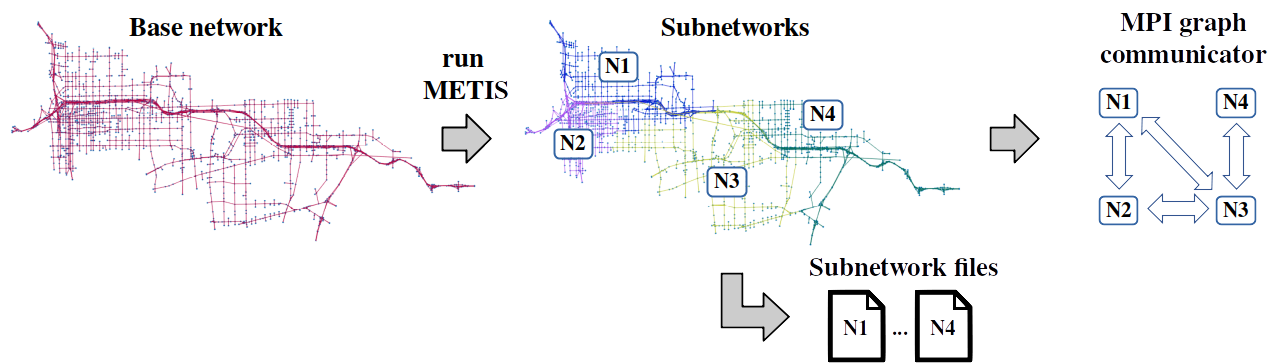
\includegraphics[width=0.9\textwidth]{figs/splitter.png}
  \caption{Network partitioning.}
  \label{fig:partition}
\end{figure*}

\subsection{Network partitioning}
The process of distributing the simulation among $n$ cores is illustrated in Figure~\ref{fig:partition}. The first step is to split the base network into $n$ subnetworks. To obtain these, the set of nodes is divided into non-overlapping sets. Let $\mathcal{N}_i$, $i\in[1\hdots n]$, denote the $i$th subset of nodes. The $i$th subnetwork contains all of the nodes in $\mathcal{N}_i$, as well as all of the links with either start or end node in $\mathcal{N}_i$. 
Links with start node in one subset and end node in another constitute the \textit{overlap} between two subnetworks. An overlap link with start node in $\mathcal{N}_i$ and end node in $\mathcal{N}_j$ is called a \textit{relative source} with respect to subnetwork $j$ and a \textit{relative sink} with respect to subnetwork $i$. The road connections that enter (exit) a relative source (sink) link are called \textit{relative source (sink) road connections} (with respect to a given subnetwork). The implementation utilizes an off-line module that invokes METIS~\cite{kaku:98a} to create the node subsets, and then constructs separate input files for each of the subnetworks. These files contain all of the information (and only that information) that is required to run the given subnetwork as a stand-alone simulation. 

\subsection{Process communication}

The connections between the $n$ subnetworks are encoded in a so-called \textit{metagraph}. This is a graph in which each vertex represents the non-overlapping portions of a subnetwork, and the edges are the relative sources and sinks. Each subnetwork is executed by a separate process. The appropriate MPI communicator for this configuration is the \textit{graph communicator}, which encodes the relations of the metagraph. An all-to-all transmission with a graph communicator exchanges messages amongst neighboring vertices in the metagraph. 

The message passed between two neighboring subnetworks consists of an array of numbers representing the vehicles that travel along all of the relative source and sink road connections that join the two subnetworks. During the initialization phase, the processes construct and exchange decoder maps with each of their neighbors. These map each position in the array to a lane group and state index. This same map is used throughout the entire simulation. The approach is conservative in the sense that the size of the message is fixed, and may contain many zeros at any given time. As is shown in Section~\ref{sec:experiments}, the communication time is a small fraction of the total run time, and hence the potential advantage of using dynamic message sizes is small.

The number of vehicles that travel at each time step over relative road connections (i.e. the flow between subnetworks) is computed by the node model in step 2. The MPI communication step is then inserted between steps 2 and 3. This completes the input and output flow computation for relative sources and sinks. After this, step 3) is executed to compute the downstream link for probabilistically routed vehicles, and then the internal state of all of the lane groups is updated. These steps are identical to their counterparts in the sequential model. Hence the result is not affected by the distribution of the calculation over multiple processes.


\subsection{Traffic modeling}
The full mathematical description of OTM can be found in~\cite{Gomes2019OTM}.
The description provided here omits certain details, but is sufficient to understand the inter-process communication that enables distributed simulation. The model is in the class of \textit{cell transmission} models first introduced by Daganzo in \cite{DaganzoCTM}. Since then there have been many extensions and improvements to the CTM, incorporating multiple lanes, non-triangular fundamental diagrams, etc. The CTM model that is implemented in OTM is adapted to an underlying representation of the road network that can be applied to the different  models in the hybrid simulation environment. As with most traffic simulators, there is a high-level graph (links and nodes) which encodes the connectivity of the road network. Each link (i.e. a segment of road between two junctions) has an internal geometry consisting of multiple lanes, turn pockets, and possibly a managed lane with access gates (in the case of a freeway link). There can also be sensors and control devices within the link. 

The relations between lanes that enter and exit a junction are defined by \textit{road connections}. A road connection indicates which lanes in an upstream link can turn into which other lanes in a downstream link. For example, a road connection may indicate that vehicles must be in the outer two lanes of the freeway in order to reach the off-ramp. The road connections that leave a link are used by the program to aggregate lanes into \textit{lane groups}. All lanes in a lane group access the same set of downstream road connections, and are therefore presumed to travel at similar speeds. In our previous example, the two outer lanes of the freeway constitute a lane group, and the remaining inner lanes are another. 

Vehicles in OTM (whether microscopic, mesoscopic, or macroscopic) are classified according to their \textit{type}. The vehicle type encodes two sets of parameters. First, it determines the vehicle's routing behavior which may be deterministic or probabilistic. Deterministically routed vehicles follow a predetermined sequence of links from their origin to their destination. Probabilistically routed vehicles direct themselves at every junction according to time-varying turning probabilities. The software supports arbitrary numbers of deterministic and probabilistic vehicle types. The second parameter of the vehicle type is a \textit{vehicle class}. The vehicle class encodes any set of parameters that the modeler wishes to prescribe. For example, it can be used to distinguish passenger vehicles from trucks (vehicle size), high-occupancy vehicles from single-occupancy vehicles (lane-usage rules), routing app equipped versus not (access to network information), etc.

In OTM's macroscopic model, each lane group is divided into a sequence of \textit{cells}. The state of each cell is the number of vehicles for each vehicle type and each downstream link. The downstream link of a vehicle is the next link in its route. This is determined in step 3) below for probabilistically routed vehicle types. Vehicles change lanes (ie move laterally between cells in adjacent lane groups) in order to reach a lane group that connects (via road connections) to its downstream link. 

The state update for each cell is executed in multiple steps, listed below. The respective formulas can be found in \cite{Gomes2019OTM}.

\vspace{1em} \noindent \textbf{1) Demand and supply calculations.} The total demand and supply for every cell are computed using the standard formulas of the cell-transmission model for a triangular fundamental diagram. For the last cell in each lane group, the demands are computed for each of the road connections that connect to the respective downstream links. Prior to computing the longitudinal demand, the model executes all lateral movements (lane changes).  

\vspace{1em}\noindent \textbf{2) Inter-link flow calculation.} The flows between links travel along road connections. The \textit{node model} resolves these flows from upstream demands and downstream supplies. The details of the node model can be found in \cite{Gomes2019OTM}. Here it will suffice to state that the output of the node model is a set of \textit{vehicle flux packets} that are delivered along road connections to downstream links. The node model ensures that the downstream links have sufficient available space to accommodate the packets.  

\vspace{1em}\noindent \textbf{3) Probabilistic routing.}
When a node has several outgoing links, probabilistically routed vehicles select which one to take according to given turning probabilities. These probabilities are sampled when the vehicle \textit{enters} the approaching link. This is in contrast with many macroscopic models where turning probabilities are sampled at the node, i.e. when the vehicle \textit{exits} the approaching link. This is done in order to improve the representation of lane changing that occurs upstream of the split.

\vspace{1em} \noindent \textbf{4) State update.} Once all packets have been received and tagged with their next downstream link, then the state of the cells can be updated using the conservation of vehicles. This calculation follows the standard cell transmission model formulas for internal cells. 

